\begin{pa} \label{PA:3.4}
According to U.S.~postal regulations, the girth plus the length of a parcel sent by mail may not exceed 108 inches, where by ``girth'' we mean the perimeter of the smallest end.  What is the largest possible volume of a rectangular parcel with a square end that can be sent by mail?  What are the dimensions of the package of largest volume? 
\begin{figure}[h]
\begin{center}
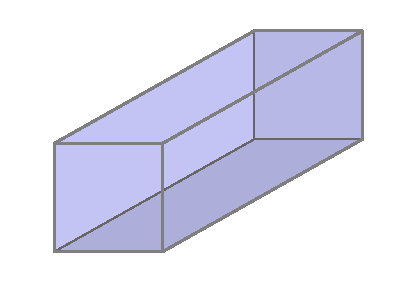
\includegraphics{figures/3_4_PA1.eps}
\caption{A rectangular parcel with a square end.} \label{F:3.4.PA1}
\end{center}
\end{figure}

\ba
	\item Let $x$ represent the length of one side of the square end and $y$ the length of the longer side.  Label these quantities appropriately on the image shown in Figure~\ref{F:3.4.PA1}.
	\item What is the quantity to be optimized in this problem?  Find a formula for this quantity in terms of $x$ and $y$.
	\item The problem statement tells us that the parcel's girth plus length may not exceed 108 inches.  In order to maximize volume, we assume that we will actually need the girth plus length to equal 108 inches.  What equation does this produce involving $x$ and $y$?
	\item Solve the equation you found in (c) for one of $x$ or $y$ (whichever is easier).
	\item Now use your work in (b) and (d) to determine a formula for the volume of the parcel so that this formula is a function of a single variable.
	\item Over what domain should we consider this function?  Note that both $x$ and $y$ must be positive; how does the constraint that girth plus length is 108 inches produce intervals of possible values for $x$ and $y$?
	\item Find the absolute maximum of the volume of the parcel on the domain you established in (f) and hence also determine the dimensions of the box of greatest volume.  Justify that you've found the maximum using calculus.
\ea
\end{pa} 
\afterpa